\documentclass[12pt]{article}
\usepackage{lecture}
\usepackage{graphics}
\usepackage{epstopdf}
\usepackage{html}
\usepackage{url}

\newcommand{\copyrightYears}{2001-2012}

\title{Mapping quantitative trait loci}

\begin{document}

\maketitle

\thispagestyle{first}

\section*{Introduction}

So far in our examination of the inheritance and evolution of
quantitative genetics, we've been satisfied with a purely statistical
description of how the phenotypes of parents are related to the
phenotypes of their offspring. We've made pretty good progress with
that. We know how to partition the phenotypic variance into genetic
and phenotypic components and how to partition the genetic variance
into additive and dominance components. We know how to predict the
degree of resemblance among relatives for any particular trait in
terms of the genetic components of variance. We know how to predict
how a trait will respond to natural selection. 

That's not bad, but in the last 20-25 years the emergence of molecular
technologies that allow us to identify large numbers of Mendelian
markers has led to a new possibility. It is sometimes possible to
identify the chromosomal location, at least roughly, of a few genes
that have a large effect on the expression of a trait by associating
variation in the trait with genotypic differences at loci that happen
to be closely linked to those genes. A locus identified in this way is
referred to as a {\it quantitative trait locus\/}, and the name given
to the approach is QTL mapping.\footnote{These notes draw heavily
  on~\cite{Lynch-Walsh-1998}}\index{quantitative trait locus}

The basic ideas behind QTL mapping are actually very simple, although
the implementation of those ideas can be quite complex. In broad
outline, this is the approach:\index{QTL mapping!outline}

\begin{itemize}

\item Produce a set of progeny of known parentage. One common design
  involves first crossing a single pair of ``inbred'' parents that
  differ in expression of the quantitative trait of interest and then
  crossing the $F_1$s, either among themselves to produce $F_2$s (or
  recombinant inbred lines) or backcrossing them to one or both
  parents.

\item Construct a linkage map for the molecular markers you're
  using. Ideally, you'll have a large enough number of markers to
  cover virtually every part of the genome.\footnote{We'll talk a
    little later about how many markers are required.}

\item Measure the phenotype and score the genotype at every marker
  locus of every individual in your progeny sample.

\item Collate the data and analyze it in a computer package like {\tt
  QTL Cartographer} to identify the position and effects of QTL
  associated with variation in the phenotypic trait you're interested
  in.

\end{itemize}

\noindent If that sounds like a lot of work, you're right. It is. But
the results can be quite informative, because they allow you to say
more about the genetic influences on the expression of the trait
you're studying than a simple parent-offspring regression.

\section*{Thoday's Method\footnote{Primarily of historical
interest, but it sets the stage for what is to follow.}} 

Suppose there is a locus, $Q$, influencing the expression of a
quantitative trait situated between two known marker loci, $A$ and
$B$.\footnote{Of course, we don't know it's there when we start, but
  as we've done so many other times in this course, we'll assume that
  we know it's there and come back to how we find out where ``there''
  is later.} If we have inbred lines with different phenotypes, we can
assume that one line has the genotype $AQB/AQB$ and the other has the
genotype $aqb/aqb$. The procedure for detecting the presence of $Q$ is
as~follows:

\begin{enumerate}

\item Cross the inbred lines to form an $F_1$. The genotype of all
$F_1$ progeny will be~$AQB/aqb$.

\item Intercross the $F_1$'s to form an $F_2$ and look at the progeny 
with recombinant genotypes, e.g., $aB/ab$.

\item If $Q$ lies between $A$ and $B$

    \begin{enumerate}

    \item The phenotypes of progeny will fall into two distinct
      classes corresponding with the genotypes: $aqB/aqb$ and
      $aQB/aqb$.\footnote{Actually there could be a third phenotypic
        class if there are two recombination events between $a$ and
        $b$, i.e., $aQB/aQb$. Thoday's method assumes that the
        recombination fraction between $A$ and $B$ is small enough
        that double recombination events can be ignored, because if we
        don't ignore that possibility we must also admit that there
        will be some $aqB/aQb$ genotypes that we can't distinguish
        from $aQB/aqb$~genotypes.}

    \item The recombination fraction between $A$ and $Q$ is related to
    the proportion of $qq$ and $Qq$ genotypes among the~progeny.

    \end{enumerate}

\end{enumerate}

\noindent Notice that in this last step we actually have a criterion
for determining whether $Q$ lies between $A$ and $B$. Namely, if $A$
and $B$ are close enough in the linkage map that there is essentially
no chance of double recombination between them, then we'll get the two
phenotype classes referred to in recombinants between $A$ and $B$. If
$Q$ lies outside this region,\footnote{More specifically, if $Q$ is
  not linked to $B$, or if $Q$ has only a small effect on expression
  of the trait we're studying.} we'll get the two phenotype classes in
1:1 proportions and associated independently with genotype differences
at the $B$ locus.\footnote{This logic not only depends on ignoring the
  possibiity of double crossovers, but also on assuming that
  individual loci influencing the quantitative trait have effects
  large enough that there will be two categories of offspring,
  corresponding to the difference between $qq$ homozygotes and $qQ$
  heterozygotres.} 


\section*{Genetic recombination and mapping functions}

Genetic mapping is based on the idea that recombination is more likely
between genes that are far apart on chromosomes than between genes
that are close. If we have three genes $A$, $B$, and $C$ arranged in
that order on a chromosome, then
\[
r_{AC} = r_{AB}(1-r_{BC}) + (1-r_{AB})r_{BC} \qquad ,
\]
where $r_{AB}$, $r_{AC}$, and $r_{BC}$ are the recombination rates
between $A$ and $B$, $A$ and $C$, and $B$ and $C$,
respectively.\footnote{In practice this isn't quite true. Interference
  may cause the recombination rate between $A$ and $C$ to differ from
  this simple prediction. That's not much of a problem since we can
  just use a mapping function that corrects for this problem, but
  we'll ignore interference to keep things~simple.}

Haldane pointed out that this relationship implies another, namely
that the probability that there are $k$ recombination events between
two loci $m$ map units apart is given by the Poisson~distribution:
\[
p(m,k) = {e^{-m} m^k \over k!} \qquad .
\]
Now to observe a recombination event between $A$ and $C$ requires that
there be an odd number of recombination events between them~(1, 3, 5,
$\ldots$), i.e.,
\begin{eqnarray*}
r_{AC} &=& \sum_{k=0}^\infty \frac{e^{-m} m^{(2k+1)}}{(2k+1)!} \\
       &=& \frac{1 - e^{-2m}}{2} \qquad .
\end{eqnarray*}
This leads to a natural definition of map units~as
\[
m = -\ln (1-2r) /2 \qquad .
\]
$m$ calculated in this way gives the map distance in Morgans
($1M$). Map distances are more commonly expressed as centiMorgans,
where $100cM = 1M$. Notice that when $r$ is small, $r \approx m$, so
the map distance in centiMorgans is approximately equal to the
recombination frequency expressed as a percentage. There are several
other mapping functions that can be chosen for an analysis. In
particular, for analysis of real data investigators typically choose a
mapping function that allows for interference in recombination. We
don't have time to worry about those complications, so we'll use only
the Haldane mapping function in our further discussions.

\section*{How many markers will you need?}

If markers are randomly placed through the genome, then the average
distance between a QTL and the closest marker~is
\[
E(m) = {L \over 2(n+1)} \qquad ,
\]
where $L$ is the total map length and $n$ is the number of markers
employed. The upper 95\% confidence limit for the distance~is
\[
{L \over 2}\left(1 - 0.05^{(1/n)}\right) \qquad .
\]
Since the human genome is 33M (3300cM), 110 random markers give an
average distance of 14.9cM and an upper 95\% confidence limit
of~44.3cM, corresponding to recombination frequencies of 0.13 and
0.29, respectively. Since there are about 30,000 genes in the human
genome, there are roughly 10 genes per centimorgan. So if you're QTL
is 44cm from the nearest marker, there are probably over 400 genes in
the chromosomal segment you've identified.

If $r_{MQ}$ is the recombination fraction between the nearest marker
locus and the QTL of interest, the frequency of recombinant genotypes
among $F_2$ progeny is $2r_{MQ}(1-r_{MQ}) + r_{MQ}^2$. As you can see
from the graph in Figure~\ref{fig:recombination}, there's a nearly
linear relationship between recombination frequency and the frequency
of recombinant phenotypes~($p$ in the graph). Think about what that
means. Having a really dense map with a lot of markers is great,
because it will allow you to map your QTL very precisely, {\it if} you
look at enough segregating offspring to have a reasonable chance of
picking up recombinants between them. With 3300cM in the human genome
and roughly 3 GB of sequence to get within 1 MB of the actual QTL,
you'd need one marker per centimorgan. To have 10 recombinants between
markers bracketing the QTL, you'd need to analyze 1000
chromosomes.\footnote{These calculations are moot in this context, of
  course. You can't ethically do a QTL study in humans. But the same
  principles apply to association mapping, which we'll get to in a
  couple of lectures.}

\begin{figure}
\begin{center}
\resizebox{!}{6cm}{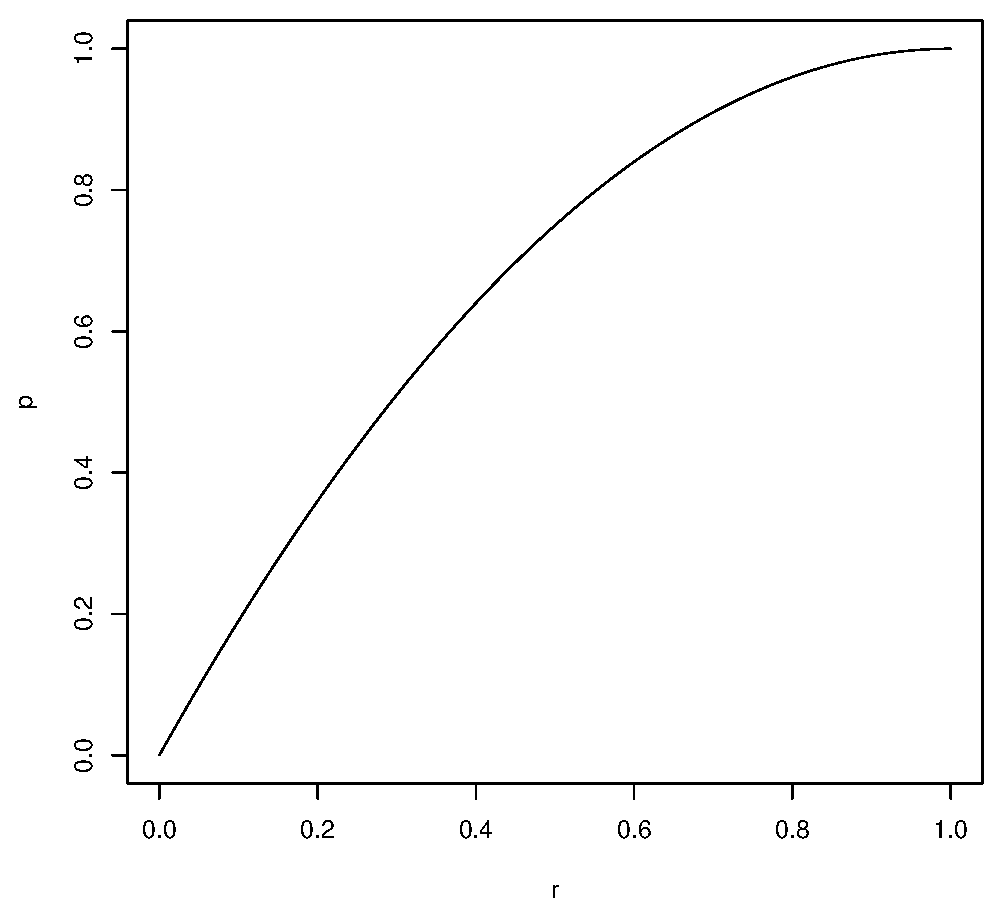
\includegraphics{recombination.eps}}
\end{center}
\caption{The relationship between recombination frequency, $r$, and
  the frequency of recombinant phenotypes, $p$, assuming a Haldane
  mapping function.}\label{fig:recombination}
\end{figure}

\section*{Analysis of an $F_2$ derived from inbred lines}\index{QTL mapping!inbred lines}

An analysis of inbred lines uses the same basic design as Thoday, but
takes advantage of more information.\footnote{As I alluded to earlier,
  other breeding designs are possible, including backcrosses and
  recombinant inbred lines and analyses involving outbred parents. The
  principles are the same in every case, but the implementation is
  different.} We start with two inbred lines $M_1QM_2/M_1QM_2$ and
$m_1qm_2/m_1qm_2$, make an $F_1$, intercross them, and score the
phenotype and marker genotype of each individual. Analysis of the data
is based on calculating the frequency of each genotype at the $Q$
locus as a function of the genotype at the marker loci and the
recombination fractions between the marker loci and $Q$.\footnote{You
  should be getting used to the idea now that we always assume we know
  something we don't and then backcalculate from what we do know to
  what we'd like to~know.} For example,
\begin{eqnarray*}
P(M_1QM_2/M_1QM_2) &=& \left((1-r_{1Q})(1-r_{Q2})/2\right)^2 \\
P(M_1QM_2/M_1qM_2) &=& 2\left((1-r_{1Q})(1-r_{Q2})/2\right)
                       \left(r_{1Q}r_{Q2}/2\right) \\
P(M_1qM_2/M_1qM_2) &=& \left(r_{1Q}r_{Q2}/2\right)^2 \qquad .
\end{eqnarray*}
Because the frequency of $M_1M_2/M_1M_2 = \left((1-r_{12})/2\right)^2$,
we can use Bayes' Theorem to write the conditional probabilities of
getting each genotype~as
\begin{eqnarray*}
P(QQ|M_1M_2/M_1M_2) &= {(1-r_{1Q})^2(1-r_{Q2})^2 \over (1-r_{12})^2} \\
P(Qq|M_1M_2/M_1M_2) &= {2r_{1Q}r_{Q2}(1-r_{1Q})(1-r_{Q2})
                       \over (1-r_{12})^2} \\
P(qq|M_1M_2/M_1M_2) &= {r_{1Q}^2 r_{Q2}^2 \over (1-r_{12})^2} 
                       \qquad .
\end{eqnarray*}
Clearly, if we wanted to we could right down similar expressions for
the nine remaing marker genotype classes, but we'll stop here. You get
the~point.\footnote{I should say, I {\it hope\/} you get the point.}

Now that we've got this we can write down the likelihood of getting
our data, namely
\[
L(x|M_j) = \sum_{k=1}^N \phi (x|\mu_{Q_k}, \sigma^2) P(Q_k|M_k) \qquad ,
\]
where $N$ is the number of QTL genotypes considered, $\phi
(x|\mu_{Q_k}, \sigma^2)$ is the probability of getting phenotype $x$
given the mean phenotype, $\mu_{Q_k}$, and variance, $\sigma^2$,
associated with $Q_k$, and $P(Q_k|M_k)$ is the probability of getting
$Q_k$ given the observed marker genotype. Fortunately, we don't have
to do any of these calculations, all we do is to ask our good
friend~(QTL Cartographer) to do the calculations for us. It will scan
the genome, and tell us how many QTL loci we are likely to have, where
they are located relative to our known markers, and what the additive
and dominance effects of the alleles are. 

\section*{The Caveats}\index{QTL mapping!caveats}

That's wonderful, isn't it? We have to do a little more work than for
a traditional quantitative genetic analysis, i.e., we have to do a
bunch of molecular genotyping in addition to all of the measurements
we'd do for a quantitative genetic experiment anyway, but we now know
how how many genes are involved in the expression of our trait, where
ther are in the genetic map, and what their additive and dominance effects
are. We can even tell something about how alleles at the different
loci interact with one another. What more could you ask for? Well,
there are a few things about QTL analyses to keep in mind.

\begin{itemize}

\item As currently implemented, QTL mapping procedures assume that the
  distribution of trait values around the genotype mean is normal,
  {\it with the same variance for all QTL~genotypes}.\footnote{I {\it
      know\/} you picked up on that when I said that the phenotypic
    variance associated with each QTL genotype was $\sigma^2$. You
    were just too polite to point it out and interrupt me.}

\item QTL mapping programs often estimate the effects of each locus
  individually. It's not at all easy to search simultaneously for the
  joint effects of two QTL loci, although it's not too hard to look at
  the combined effects of QTL loci first identified
  individually. Composite interval mapping, in which additional
  markers are included as cofactors in the analysis, partially
  addresses this limitation. Multiple interval mapping looks at
  several QTLs simultaneously and shows some promise, but as you may
  be able to imagine it's pretty hard to search for more than a few
  QTLs simultanously.

\item If some loci in the ``high'' line have ``low'' effects and vice
  versa, the effects of both loci~(and possibly other loci) may
  be~masked.

\item Using this approach we can identify the QTL's that are important
  {\it in a particular cross}, but different crosses can identify
  different QTL's. Even the same cross may reveal different QTL's if
  the measurements are done in different environments. Methods to
  analyzes several progeny sets simultaneously are only now
  being~developed.

\end{itemize}

\bibliography{popgen}
\bibliographystyle{plain}

\ccLicense

\end{document}



